\section{}
\[
H(s)=\frac{10\sqrt{2}\,s^{2}}{s-1}\,.
\]
\subsection{Bode-Diagramm}
\begin{center}
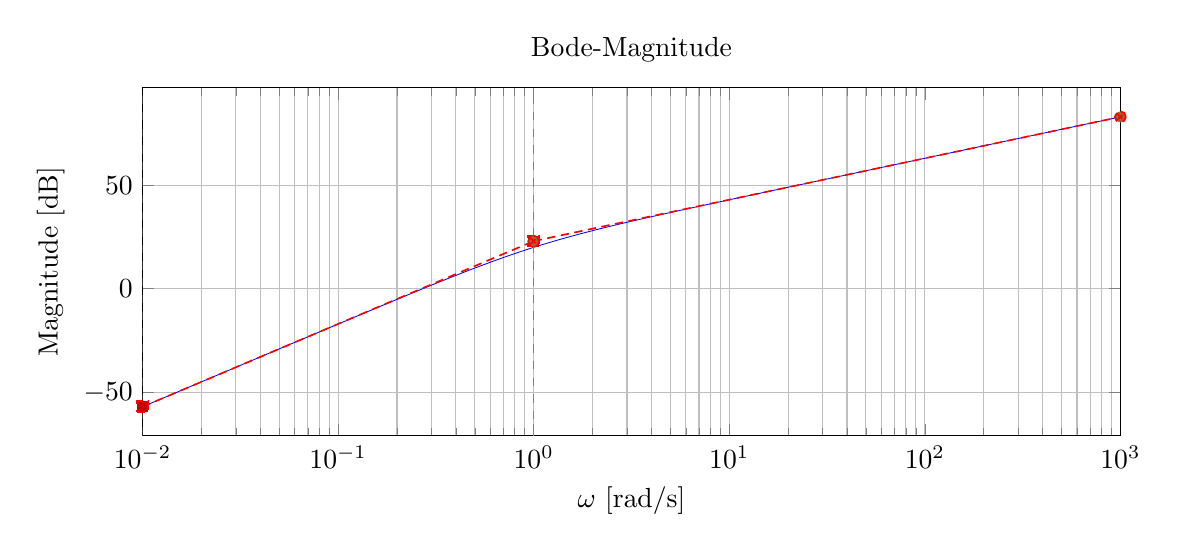
\begin{tikzpicture}
\begin{semilogxaxis}[
  width=14cm,height=6cm,
  xmin=1e-2,xmax=1e3,
  xlabel={$\omega$ [rad/s]},
  ylabel={Magnitude [dB]},
  grid=both,
  title={Bode-Magnitude}
]
\addplot[
  domain=1e-2:1e3,
  samples=600,
  mark=none,
  line width=0.3pt,
  blue
] {20 + 10*ln(2)/ln(10) + 40*ln(x)/ln(10) - 10*ln(1 + x^2)/ln(10)};
\addplot+[domain=1e-2:1,samples=2,dashed,dash pattern=on 3pt off 2pt,line width=0.6pt,red] {20 + 10*ln(2)/ln(10) + 40*ln(x)/ln(10)};
\addplot+[domain=1:1e3,samples=2,dashed,dash pattern=on 3pt off 2pt,line width=0.6pt,red] {20 + 10*ln(2)/ln(10) + 20*ln(x)/ln(10)};
\draw[gray,dashed] (rel axis cs:0,0) -- (rel axis cs:0,1);
\draw[gray,dashed] (axis cs:1,\pgfkeysvalueof{/pgfplots/ymin}) -- (axis cs:1,\pgfkeysvalueof{/pgfplots/ymax});
\node[gray,anchor=south east] at (axis cs:1,\pgfkeysvalueof{/pgfplots/ymax}) {\scriptsize Pol $\omega_p=1$ (RHP)};
\end{semilogxaxis}
\end{tikzpicture}
\vspace{6mm}
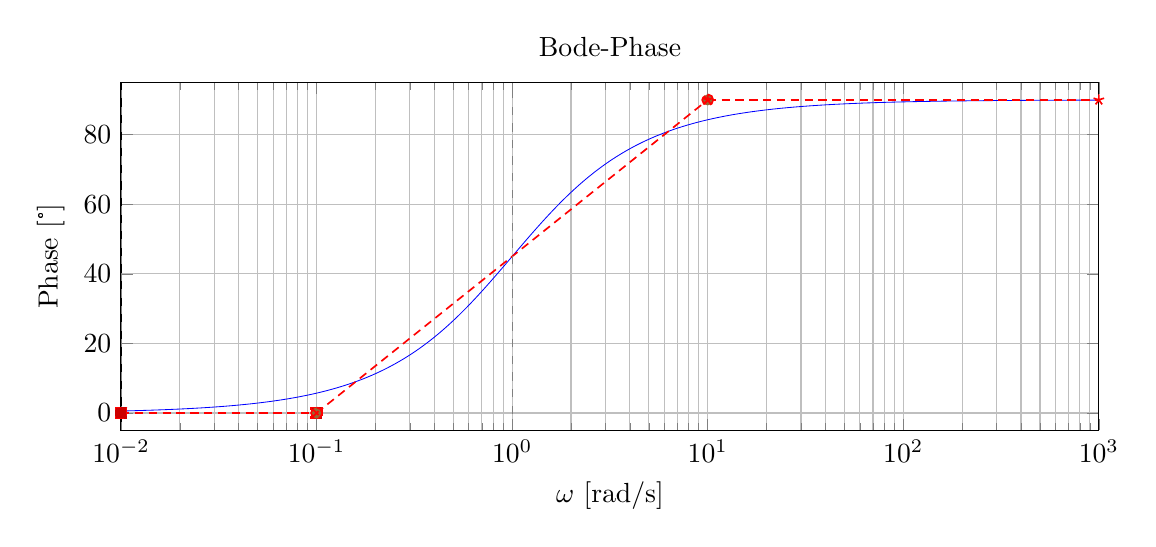
\begin{tikzpicture}
\begin{semilogxaxis}[
  width=14cm,height=6cm,
  xmin=1e-2,xmax=1e3,
  ymin=-5,ymax=95,
  xlabel={$\omega$ [rad/s]},
  ylabel={Phase [°]},
  grid=both,
  title={Bode-Phase}
]
\addplot[
  domain=1e-2:1e3,
  samples=600,
  mark=none,
  line width=0.3pt,
  blue
] {atan(x)};
\addplot+[domain=1e-2:1e-1,samples=2,dashed,dash pattern=on 3pt off 2pt,line width=0.6pt,red] {0};
\addplot+[domain=1e-1:1e1,samples=2,dashed,dash pattern=on 3pt off 2pt,line width=0.6pt,red] {45 + 45*ln(x)/ln(10)};
\addplot+[domain=1e1:1e3,samples=2,dashed,dash pattern=on 3pt off 2pt,line width=0.6pt,red] {90};
\draw[gray,dashed] (rel axis cs:0,0) -- (rel axis cs:0,1);
\draw[gray,dashed] (axis cs:1,\pgfkeysvalueof{/pgfplots/ymin}) -- (axis cs:1,\pgfkeysvalueof{/pgfplots/ymax});
\node[gray,anchor=south east] at (axis cs:1,\pgfkeysvalueof{/pgfplots/ymax}) {\scriptsize Pol $\omega_p=1$ (RHP)};
\end{semilogxaxis}
\end{tikzpicture}
\end{center}
\newpage
\subsection{Erklärung}
\vspace{5mm}
\begin{description}[leftmargin=1.2em,labelsep=.6em,font=\bfseries]
\item[Schritt 1] Doppelnullstelle im Ursprung: $H(s)=10\sqrt{2}\,\dfrac{s^2}{s-1}$. Für $\omega\ll1$ gilt $|H(\j\omega)|\approx 10\sqrt{2}\,\omega^{2}$; Startsteigung $+40\,\mathrm{dB/dec}$. Phasenlage bei sehr kleinen $\omega$: $\angle(\j\omega)^2=+180^\circ$, der Nenner $\j\omega-1\approx-1$ trägt $+180^\circ$ bei; Differenz kompensiert $\Rightarrow$ Startphase $\approx0^\circ$.
\item[Schritt 2] Rechter-Halbraum-Pol bei $\omega_p=1\,\mathrm{rad/s}$ (nicht-minimumphasig): Magnitudenbeitrag identisch zum LHP-Pol. Ab $\omega=1$ wird die Slope um $-20\,\mathrm{dB/dec}$ reduziert, damit gesamt $+20\,\mathrm{dB/dec}$ für $\omega\gg1$. Eckpunktexaktwert: $|H(\j1)|=10\Rightarrow 20\,\mathrm{dB}$, also $-10\log_{10}2\approx-3.01\,\mathrm{dB}$ unter der Geradennäherung. Phasenverlauf des RHP-Pols: Anstieg von $0^\circ$ auf $+90^\circ$ über die Übergangsdekade $\omega\in[0.1,10]$; Geradennäherung $\varphi_{\text{approx}}(\omega)=45^\circ+45^\circ\log_{10}\omega$ in $[0.1,10]$, mit $\angle H(\j1)=+45^\circ$.
\item[Schritt 3] Grenzverhalten: Für $\omega\ll1$ gilt $|H(\j\omega)|_{\mathrm{dB}}\approx 20+10\log_{10}2+40\log_{10}\omega$ und $\angle H\approx0^\circ$. Für $\omega\gg1$ folgt $|H(\j\omega)|_{\mathrm{dB}}\approx 20+10\log_{10}2+20\log_{10}\omega$ (Netto-Slope $+20\,\mathrm{dB/dec}$), die Phase nähert sich $+90^\circ$.
\end{description}

\vspace{0.5cm}
\medskip
\noindent\textbf{Stückweise Näherung}
\[
|H(\j\omega)|_{\mathrm{dB}}\approx
\begin{cases}
20+10\log_{10}2+40\log_{10}\omega,& \omega\ll1,\\[4pt]
\left.\;20+10\log_{10}2\;\right.-10\log_{10}2=20,& \omega=1,\\[4pt]
20+10\log_{10}2+20\log_{10}\omega,& \omega\gg1,
\end{cases}
\qquad
\]
\newpage